%% content.tex
%%

%% ==============================
\chapter{Prelude}
\label{ch:Introduction}
%% ==============================

\section{Abstract}

\section{Einleitung}


%% ==============
\chapter{Grundlagen}
\label{ch:Grundlagen}
%% ==============


%% ===========================
\section{Path Tracer}
\label{ch:Content1:sec:Path Tracer}
\subsubsection{Funktionsweise}
Bei der Bilderzeugung, ausgehend von Szenen, welche viel Geometrie beinhalten bzw. bei Szenen 
die generelle BRDF's verwenden eignet sich das \ref{ch:Content1:sec:PathTracer}path tracing \cite{kajiya1986rendering}.
Das \ref{ch:Content1:sec:PathTracer}path tracing ist in Hinsicht der Beleuchtung komplett. Deshalb lässt sich damit
\textit{Global Illumination} erreichen. Das hier verwendete \ref{ch:Content1:sec:PathTracer}path tracing in 
\cite[eragae]{Benty18} verwendet eine klassische Umsetzung.\par

\begin{figure}[H]
    \centering
    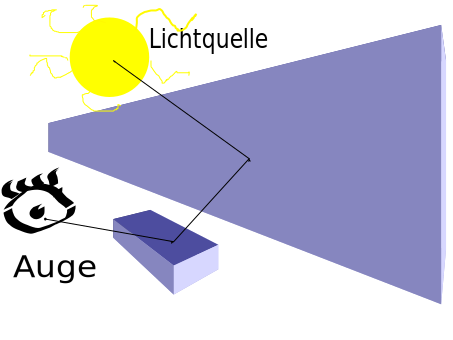
\includegraphics[width=0.7\linewidth]{content/PathTracer/Bilder/Grundkonzept_path_tracing.pdf}
    \label{pic::PathTracingGrundkonzept}
    \caption{Grundkonzept path tracer}
\end{figure}


Wie in \cite{marschner2009fundamentals} beschrieben wird ausgehend von der vollständigen Transportgleichung
\begin{equation}\label{eq:vollstaendige Transportgleichung}
    L_s(k_0) = L_e(k_0) + \int_{all(k_i)}^{} \rho(k_i, k_0)*L_f(k_i)*cos(\theta_i)d\theta_i
\end{equation}
    
\begin{equation}\label{eq:kajiya}
        I(x,{x}^{'}) = g(x,{x}^{'}) * \biggl[\epsilon(x,{x}^{'}) + 
                        \int_{S}^{} \rho(x,{x}^{'},{x}^{''})
                        I({x}^{'},{x}^{''}d{x}^{''})\biggr] 
\end{equation}
Sie beschreibt den Energietransport \textit{I} von einem Punkt ${x}^{'}$
zu einem Punkt x. Dabei ist ein maßgebender Faktor der Geometrieterm \textit{g},
der die relative Lage der beiden Punkte zueinander im Raum beschreibt.
Ein weiterer Faktor ist die Abstrahlung \textit{$\epsilon$} von ${x}^{'}$ nach x. 
Beeinflusst wird der Energiefluss auch durch
die bidirektionale Verteilungsfunktion \textit{$\rho$}, welche Aufschluss über
das einfallende Licht von einem Punkt ${x}^{''}$ über ${x}^{'}$ zu x gibt.\par
Die Schlussfolgerung aus dieser Gleichung \ref{eq:kajiya} ist: Die transportierte
Intensität von einem Licht zu einem Anderen ist die Summe des ausgestrahlten Lichts 
und das ausgestrahlte Licht zu x von allen anderen Oberflächen.


\subsubsection{Monte-Carlo-Integration}
Mit der Monte Carlo Integration approximieren wir die Rendergleichung.\par 
Bei gegebener Funktion \textit{f }:\textit{ S}$\rightarrow \mathbb{R}$ und der 
Wahrscheinlichkeitsdichtefunktion $x \sim p$
\cite{KK02}
\label{pic:MonteCarloIntegration}
\begin{equation}\label{eq:montcarlo}
    \int_{x\in S} g(x) d\mu \simeq \frac{1}{N}*\sum_{i=1}^{N}\frac{g(x_i)}{p(x_i)}
\end{equation}

\begin{figure}[H]\label{pic:WeissesRauschenTracer}
    \centering
    \begin{minipage}[t]{0.45\linewidth}
        \centering
        \includegraphics[width=\linewidth]{content/PathTracer/Bilder/WeissesRauschenSzene.png}
        \caption{Szene mit Weißem Rauschen}
    \end{minipage}
    \hfill
    \begin{minipage}[t]{0.45\linewidth}
        \centering
        \includegraphics[width=\linewidth]{content/PathTracer/Bilder/FFT_Ausschnitt2.png}
        \caption{FFT des Ausschnitts}
    \end{minipage}
\end{figure}




%% ===========================

\dots


%% ===========================
\section{Blue Noise}
\label{ch:Content1:sec:BlueNoise}
\subsection{Eigenschaften}

Wie in \cite{Pet17} vorgestellt, macht man sich die Eigenschaften einer
blue noise Textur zu Nutze. Dabei werden im Folgenden, die dort bereit 
gestellten blue noise verteilten Texturen verwendet, welche anhand des in
\cite{ulichney1993void} vorgestellten Algorithmus erstellt wurden.
Die korrespondierenden Spektren werden mit Hilfe von \cite{FFTProgWeb} erstellt.

\subsubsection{Uniformität}
Die Uniformität(lat. \textit{uniformitas}-Einförmigkeit) garantiert uns 
wie in \cite{3288} eine gleichverteilte Wahrscheinlichkeitsdichtefunktion
mit zugehöriger gleichverteilter Wahrscheinlichkeitsfunktion. In \cite{Pet17}
sieht sie wie folgt aus: 

\begin{equation}\label{eq:uniformität}
    P(n \leq p) = p
\end{equation}

\subsubsection{Niedrige Frequenzen}
Niedrige Frequenzen sind in einer blue noise sehr wenig bis gar nicht 
vertreten. Dies ist an dem schwarzen Ring innerhalb der Fouriertransformierten
zu erkennen\ref{pic:blueNoiseFFT}.

\begin{figure}[H]\label{pic:blueNoiseFFT}
    \centering
    \begin{minipage}[t]{0.45\linewidth}
        \centering
        \includegraphics[width=\linewidth]{content/BlueNoise/Bilder/LDR_LLL1_0.png}
        \caption{$512^{2}$ blue noise Textur}
    \end{minipage}
    \hfill
    \begin{minipage}[t]{0.45\linewidth}
        \centering
        \includegraphics[width=\linewidth]{content/BlueNoise/Bilder/FFT_LDR_LLL1_0.png}
        \caption{Fourier Spektrum $512^{2}$ blue noise Textur}
    \end{minipage}
\end{figure}

\begin{figure}[H]\label{pic:bayerPatternFFT}
    \centering
    \begin{minipage}[t]{0.45\linewidth}
        \centering
        \includegraphics[width=\linewidth]{content/BlueNoise/Bilder/BayerMatrix.png}
        \caption{$512^{2}$ bayer pattern Textur}
    \end{minipage}
    \hfill
    \begin{minipage}[t]{0.45\linewidth}
        \centering
        \includegraphics[width=\linewidth]{content/BlueNoise/Bilder/FFT_BayerMatrix.png}
        \caption{Fourier Spektrum $512^{2}$ bayer pattern Textur}
    \end{minipage}
\end{figure}

\begin{figure}[H]\label{pic:tiledBlueNoiseFFT}
    \centering
    \begin{minipage}[t]{0.45\linewidth}
        \centering
        \includegraphics[width=\linewidth]{content/BlueNoise/Bilder/BlueNoise64Tiled.png}
        \caption{$512^{2}$ bayer pattern Textur}
    \end{minipage}
    \hfill
    \begin{minipage}[t]{0.45\linewidth}
        \centering
        \includegraphics[width=\linewidth]{content/BlueNoise/Bilder/FFT_BlueNoise64Tiled.png}
        \caption{Fourier Spektrum $512^{2}$ bayer pattern Textur}
    \end{minipage}
\end{figure}

\subsubsection{Isotropie}
Die Isotropie(altgr. \textit{isos}-gleich und \textit{tropos}-Richtung)
einer blue noise Textur wird ausgenutzt. Dabei haben wir in allen
Dimensionen (in dieser Arbeit werden Texturen mit zwei benutzt) 
die Unabhängigkeit einer Eigenschaft. 


\subsubsection{Kachelung}
Eine weitere nützliche Eigenschaft der blue noise Verteilung ist die 
Möglichkeit der Kachelung. 
%% ===========================

\dots


%% content.tex
%%

%% ==============
\chapter{Temporaler Algorithmus}
\label{ch:Content2}
%% ==============

\dots


%% ===========================
\section{Sorting}
\label{ch:Content2:sec:Sorting}
In diesem Schritt wollen wir nun die Untersuchungen aus 
\ref{ch:Content2:sec:APosteriori} durchführen. Nach dem Rendern eines
Frames t(vor dem Rendern von Frame t+1) approximieren wir das Histogramm
der Pixelwerte anhand der Pixelwerte von Frame t.
\cite{hal02158423}
\begin{algorithm}[H]
    \caption{\textbf{Sortier Schritt t} nach dem Rendern von Frame t
    und vor dem Rendern von Frame t+1}
    \begin{algorithmic}[1]
        \STATE pixel \textbf{consists of} value,index;
        \STATE List framePixelsIntensities, noiseIntensities;
        \STATE $assert(sizeof(framePixelsIntensities)==BLOCKSIZE)$;
        \STATE $assert(sizeof(noiseIntensities)==BLOCKSIZE)$;
        \STATE List L $\leftarrow$ pixels of frame t in block;
        \STATE \hfill
        \STATE //init lists
        \STATE initList(framePixelsIntensities, pixelIntensity(L);
        \STATE $blueNoise_{t}$ = calcCorrectOffset(incomingbluenoisetexture);
        \STATE initList(noiseIntensities, pixelIntensity($blueNoise_{t}$));
        \STATE \hfill
        \STATE //sort the two lists by means of intensities
        \STATE sort(framePixelsIntensities);
        \STATE Sort(noiseIntensities);
        \STATE \hfill
        \STATE //now we reorder our seeds hence the sorted lists
        \FORALL{$i = 1 .. BLOCKSIZE$}
        \STATE $sortedSeeds(noiseIntensities.getIndex(i)) = incomingSeeds(framePixelIntensities.getIndex(i))$;
        \ENDFOR
    \end{algorithmic}
    \label{alg:Sortier}
\end{algorithm}
%% ===========================

\dots


%% ===========================
\section{Retargeting}
\label{ch:Content2:sec:Retargeting}
\cite{hal02158423}

Zu Grunde liegender Sinn dieses Schrittes: Vertauschen der Anfangswerte, die 
verteilt sind wie $BlueNoise_{t}$, sodass Sie verteilt sind wie die 
$BlueNoise_{t+1}$. Aufgrund dessen haben wir eine Aufsummierung der
blue noise Fehlerverteilungen über viele Frames.

\begin{algorithm}[H]
    \caption{\textbf{Retargeting Schritt} t Vor Rendern Frame t+1 nach Sortier Schritt}
    \begin{algorithmic}[1]
        \State //permutation indices from precomputed texture
        \State $retaget_{t}$ = retargettexure[calcCorrectOffset(incomingbluenoisetexture)];
        \State List<PixelPermutation> L = $retaget_{t}$
        \For{i = 1 .. numberOfPixelsPerBlock}
        \State $retargetedSeeds(L.getNewIndices()) = incomingSeeds(L.getOldIndices());$
        \EndFor
    \end{algorithmic}
    \label{alg:retargeting}
\end{algorithm}

%% ===========================

\dots
